%
% latex template for SAS documentation 
% name: sas.tex 
% date last modified: 8 mar 2018
% modified by: jerry 
% 
%
\documentclass{article}

\usepackage{caption}
\usepackage[margin=1in]{geometry}
\usepackage{graphicx}
\usepackage{hyperref}
\usepackage{float}
\usepackage{tabularx}
\usepackage{titling}

\begin{document}

\title{
	
\includegraphics{images/um_logo.png} \\
	\vspace{0.1in}
	CSC431 \\
	\vspace{0.2in}
	\textbf{Download of Public-facing Data} \\
	\large System Architecture Specification \\
	Team \#3
}

\author{
	Jerry Bonnell
	\and Gururaj Shriram
	\and Re Chang
	\and Heyu Yao
	\and Lixiong Liang
}

\date{}
\maketitle

\clearpage
\section*{Version History}

\begin{tabularx}{\textwidth}{| l | l | X | l |}
	\hline
	\textbf{Version} & \textbf{Date} & \textbf{Author(s)} & \textbf{Change Comments} \\
	\hline
	1 & \today & Jerry Bonnell & First Draft \\
	\hline
\end{tabularx}

\clearpage
\tableofcontents

\clearpage
\listoffigures
\listoftables

\clearpage

\section{System Analysis}

\subsection{System Overview}

Describe the system in brief and your architecture choice.

\subsection{System Diagram}

Insert System Diagram.

\subsection{Actor Identification}

Identify all actors interacting with the system.

\subsection{Design Rationale}

\subsubsection{Architectural Style}

Identify and briefly explain the architectural style, e.g. 3-tier architecture. 

\subsubsection{Design Pattern(s)}

Identify the design pattern(s) you have deemed applicable to this architecture.

\subsubsection{Framework}

Identify and briefly explain the frameworks you are using, if any. Also 
specify the rationale behind selecting this framework. 

\clearpage

\section{Functional Design}

Identify all significant workflows as sequence diagrams using the following format. 

\subsection{Diagram Title}

\begin{figure}[H]
	\begin{center}
		\caption{Diagram Title}
		\label{}
		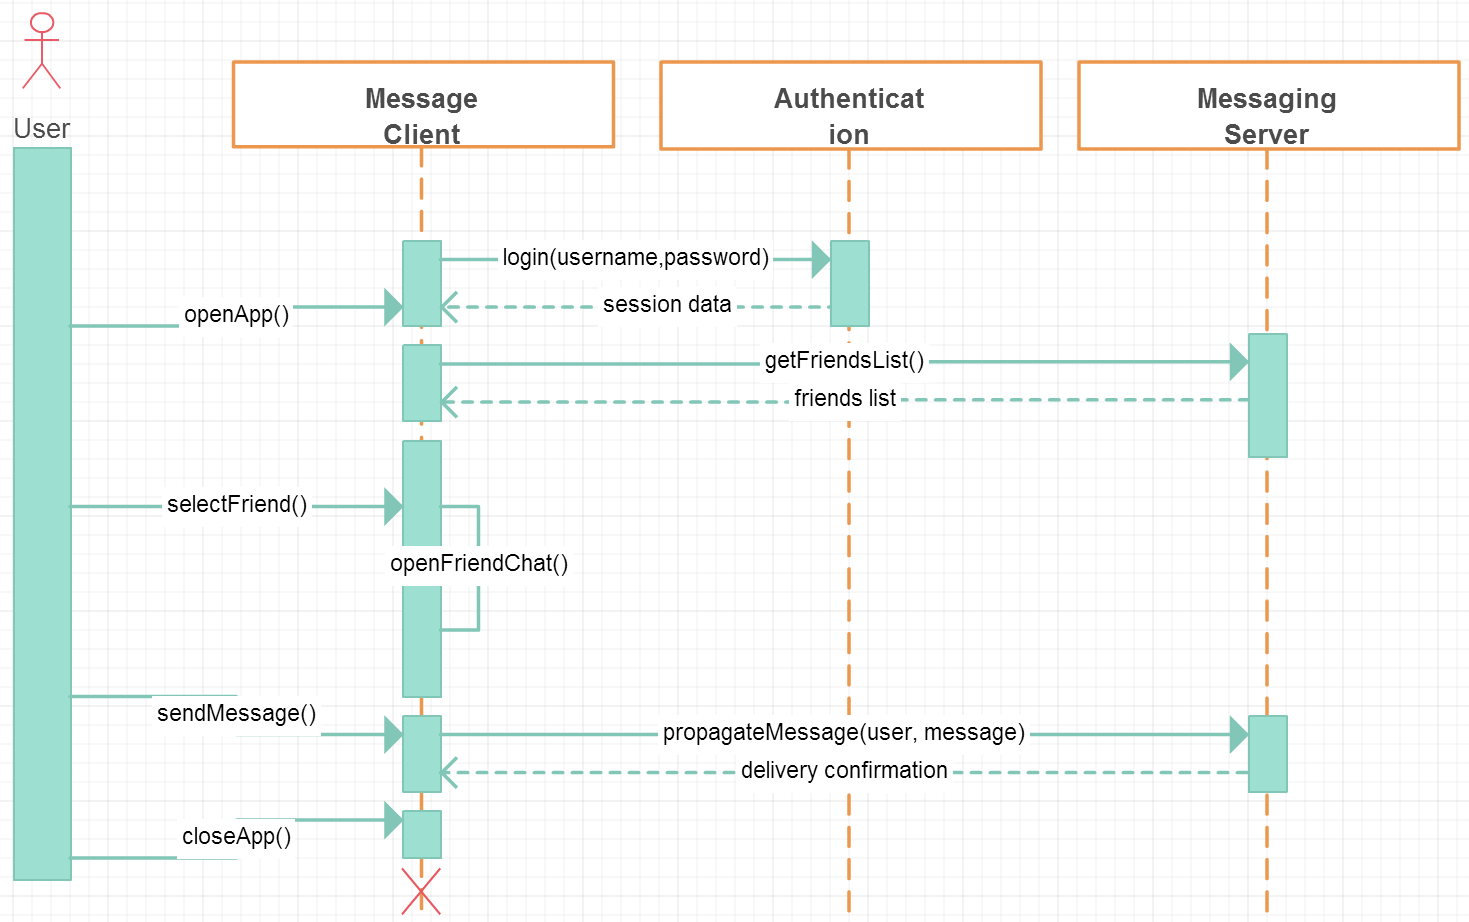
\includegraphics[width=\textwidth]{images/sample-sequence-diagram.png}
	\end{center}
\end{figure}

\clearpage

\section{Structural Design}

Identify all components and model them using class diagrams.

\end{document}
